\documentclass{beamer}

% ========== 主题 ==========
\usecolortheme{seahorse}
\useinnertheme[shadow]{rounded}
\useoutertheme[subsection=false]{smoothbars}
\setbeamertemplate{caption}[numbered]
\setbeamercovered{transparent=15}
\setbeamersize{text margin left=0.55cm, text margin right=0.55cm}

% ========== 中文与字体 (TeXLive 内置, Overleaf 可直接编译) ==========
\usepackage{xeCJK}
\setCJKmainfont{FandolSong-Regular.otf}[BoldFont=FandolSong-Bold.otf]
\setCJKsansfont{FandolHei-Regular.otf}[BoldFont=FandolHei-Bold.otf]
\setCJKmonofont{FandolFang-Regular.otf}
\setmainfont{texgyretermes-regular.otf}[BoldFont=texgyretermes-bold.otf, ItalicFont=texgyretermes-italic.otf]
\setsansfont{texgyreheros-regular.otf}[BoldFont=texgyreheros-bold.otf]
\setmonofont{texgyrecursor-regular.otf}[BoldFont=texgyrecursor-bold.otf]
\usefonttheme{serif}
\setbeamerfont{title}{family=\rmfamily,series=\bfseries}
\setbeamerfont{subtitle}{family=\rmfamily}
\setbeamerfont{date}{size=\small}
\setbeamerfont{frametitle}{family=\rmfamily,series=\bfseries,size=\large}
\setbeamerfont{framesubtitle}{family=\rmfamily,size=\small}

\usepackage{ragged2e}
\renewcommand{\raggedright}{\leftskip=0pt \rightskip=0pt plus 0cm}

% ========== 宏包与统一柔和紫系配色 ==========
\usepackage{amsmath}
\usepackage{graphicx}
\graphicspath{{./figures/}{./}}
\usepackage{booktabs}
\usepackage{xcolor}
\usepackage{tikz}
\usetikzlibrary{positioning,arrows.meta,shapes.geometric}

\definecolor{pdeep}{HTML}{5B3896}
\definecolor{pmid}{HTML}{8E73BF}
\definecolor{plight}{HTML}{F4F0FA}
\definecolor{pborder}{HTML}{C9BCE6}
\definecolor{prose}{HTML}{B54684}
\definecolor{pblue}{HTML}{4E67B0}
\definecolor{pink}{HTML}{241B35}
\definecolor{pmuted}{HTML}{6B5E80}

% ========== 元信息 ==========
\title[LMArena 选票中的形式偏向与排名失真]
{LMArena 评测选票中的回答形式偏向与排名失真}
\author[刘依然 \and 陈嘉诚 \and 韦静妍]
{刘依然 \and 陈嘉诚 \and 韦静妍}
\institute[上海财经大学]
{数据分析与可视化 · 课程期末项目\\ 上海财经大学}
\date{\today\\[0.45em]
  \href{https://github.com/lllyrrrrr/arena_project}{\textcolor{black!45}{\footnotesize\ttfamily https://github.com/lllyrrrrr/arena\_project}}}

\begin{document}

% ==================================================
% P1 封面
% ==================================================
\begin{frame}
  \titlepage
\end{frame}

% ==================================================
% P2 目录
% ==================================================
\begin{frame}{目录}
  \centering
  \begin{tikzpicture}[x=1cm,y=1cm,inner sep=0pt,outer sep=0pt]
    \foreach \chaptername/\firstp/\lastp [count=\num] in {
      背景与问题定义/3/5,
      数据清洗与口径/6/7,
      数据分析与可视化/8/17,
      {验证、讨论与反思}/18/20
    }{
      \pgfmathsetmacro{\yy}{-1.48*(\num-1)}
      \begin{scope}[shift={(0,\yy)}]
        \path[fill=plight,draw=pborder,line width=.68pt]
          (0,-.54) -- (8.94,-.54) -- (9.14,-.34)
          -- (9.14,.54) -- (.20,.54) -- (0,.34) -- cycle;
        \draw[pborder,line width=.68pt]
          (3.90,.255) -- (4.26,.255)
          (4.88,.255) -- (5.24,.255);
        \node[font=\footnotesize\bfseries,text=pink] at (4.57,.255)
          {\hyperlink{Navigation\firstp}{\num}};
        \node[font=\normalsize\bfseries,text=pink] at (4.57,-.205)
          {\hyperlink{Navigation\firstp}{\chaptername}};
      \end{scope}
    }
  \end{tikzpicture}
\end{frame}

% ==================================================
\section{背景与问题定义}
% ==================================================

% P3 背景引入
\begin{frame}{研究背景：从盲测投票到 LMArena 排行榜}
  \begin{columns}[T,onlytextwidth]
    \begin{column}{.373\textwidth}
      \footnotesize
      \linespread{1.08}\selectfont
      \setlength{\leftmargini}{1.0em}
      \setlength{\leftmarginii}{0.74em}
      \setbeamerfont{itemize/enumerate subbody}{size=\scriptsize}
      \setbeamertemplate{itemize subitem}{\raisebox{0.18ex}{\scalebox{0.68}{\textbullet}}}
      \begin{itemize}
        \setlength{\itemsep}{0.48em}
        \setlength{\rightskip}{0pt plus 1fil}
        \item 请 ChatGPT 给论文找灵感，它列了两组，再问「\textbf{\mbox{你更喜欢哪个回答？}}」
        \par\vspace{0.32em}
        \item \textbf{LMArena}（原 \mbox{Chatbot Arena}）\newline 用双答盲测给模型排名。
          \par\vspace{0.15em}
          \begin{itemize}
            \setlength{\itemsep}{0.42em}
            \setlength{\rightskip}{0pt plus 1fil}
            \item 两个匿名模型\mbox{回答同一道题}
            \item A 胜 · B 胜 · 平局 · \mbox{两边都差}
            \item 用 \href{https://proceedings.mlr.press/v235/chiang24b.html}{Bradley--Terry 模型}\mbox{汇总选票}
          \end{itemize}
      \end{itemize}
    \end{column}
    \begin{column}{.611\textwidth}
      \centering
      \includegraphics[width=\linewidth]{chatgpt_title_feedback.png}\par
      \smallskip
      {\scriptsize\color{pmuted}ChatGPT 双答\href{https://doi.org/10.1093/ijlit/eaag012}{（2026）}\par}
    \end{column}
  \end{columns}

  \vspace{0.38em}
  \begin{columns}[c,onlytextwidth]
    \begin{column}{.373\textwidth}
      \footnotesize
      \linespread{1.08}\selectfont
      \setlength{\leftmargini}{1.0em}
      \begin{itemize}
        \setlength{\rightskip}{0pt plus 1fil}
        \item Arena 把许多场匿名对局的\newline 投票汇总起来，形成公开榜单。
      \end{itemize}
    \end{column}
    \begin{column}{.611\textwidth}
      \centering
      \href{https://arena.ai}{\includegraphics[width=\linewidth]{arena_profile.png}}
    \end{column}
  \end{columns}
\end{frame}

% P4 跨年现象与文献前提
\begin{frame}{2024-2025变化：更短的提问，更长的回答}
  \vspace{0.4em}
  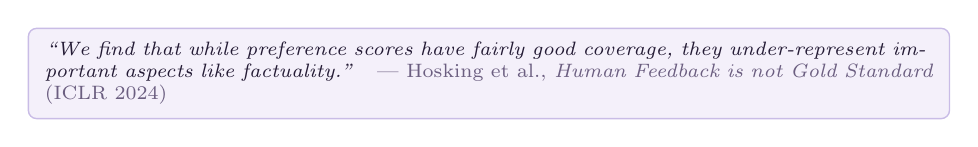
\begin{tikzpicture}
    \node[rectangle, rounded corners=3pt, fill=plight, draw=pborder, line width=0.5pt,
          text width=0.93\textwidth, inner xsep=6pt, inner ysep=5pt, font=\scriptsize, text=pink] {%
      \textit{``We find that while preference scores have fairly good coverage, they under-represent important aspects like factuality.''}
      \hfill{\color{pmuted}--- Hosking et al., \textit{Human Feedback is not Gold Standard} (ICLR 2024)}%
    };
  \end{tikzpicture}
  \vfill
  \begin{columns}[c,onlytextwidth]
    \begin{column}{0.5\textwidth}
      \centering
      \includegraphics[width=\linewidth]{fig0_length_drift.pdf}
    \end{column}
    \begin{column}{0.5\textwidth}
      \centering
      \includegraphics[width=\linewidth]{fig1_format_drift.pdf}
    \end{column}
  \end{columns}
  \vfill
  \centering
  {\footnotesize\color{pink}
    提问中位数 $143\to 94$ 字（$-34\%$）\quad$\mid$\quad
    回答中位数 $1{,}426\to 2{,}617$ 字（$\times 1.84$）\quad \quad
    主观偏好 $\neq$ 客观正确
  }
  \vspace{0.4em}
\end{frame}

% P5 核心问题与分析脉络
\begin{frame}{核心问题与分析脉络}
  \centering
  \begin{tikzpicture}[
    qboxa/.style={
      rectangle, rounded corners=4pt, fill=plight, draw=pborder, line width=0.8pt,
      text=pink, text width=10.85cm, align=center, font=\footnotesize,
      inner xsep=8pt, inner ysep=5.5pt
    },
    qboxb/.style={
      rectangle, rounded corners=4pt, fill=pdeep, text=white,
      text width=10.85cm, align=center, font=\footnotesize,
      inner xsep=8pt, inner ysep=6.5pt
    },
    stepbox/.style={
      rectangle, rounded corners=3pt, fill=plight!70, draw=pborder,
      line width=0.55pt, minimum width=10.45cm, minimum height=0.54cm, inner sep=0pt
    },
    stepnum/.style={
      circle, fill=pmid, text=white, font=\scriptsize\bfseries, inner sep=1.7pt
    },
    steptitle/.style={anchor=west, text=pink, font=\scriptsize\bfseries, inner sep=0pt},
    stepbody/.style={anchor=west, text=pmuted, font=\scriptsize, inner sep=0pt},
    arr/.style={-{Stealth[length=4.5pt,width=3.8pt]}, draw=pdeep, line width=0.95pt}
  ]
    % ===== 两个递进的核心问题（浅紫 -> 进而 -> 深紫） =====
    \node[qboxa] (q1) {%
      \textbf{核心问题}：回答的篇幅与排版，如何影响盲测投票的胜负结果？%
    };
    \node[qboxb, below=0.46cm of q1] (q2) {%
      这种形式偏好被系统性放大后，基于主观投票的公开榜单，\\%
      是否正在偏离衡量模型真实能力的初衷？%
    };
    \draw[arr] (q1.south) -- (q2.north)
      node[midway, fill=white, rounded corners=2pt, inner xsep=4pt, inner ysep=1pt,
           font=\scriptsize\bfseries, text=pdeep] {更进一步};

    % ===== 五步分析脉络（右对齐 q2，左侧独立序号轴） =====
    \node[stepbox, below=0.36cm of q2.south east, anchor=north east] (s1) {};
    \node[stepbox, below=0.14cm of s1] (s2) {};
    \node[stepbox, below=0.14cm of s2] (s3) {};
    \node[stepbox, below=0.14cm of s3] (s4) {};
    \node[stepbox, below=0.14cm of s4] (s5) {};

    \foreach \i/\t/\b in {
      1/数据清洗/对齐取样时段，剔除代码对排版计数的干扰，再按票型分组。,
      2/盲测偏好/用 Bradley--Terry 模型估计篇幅、排版与盲测胜率的关联。,
      3/名次变动/对照调整前后的模型名次，比较两期榜单的变动幅度。,
      4/题型与票型/按题型和篇幅差距比较胜率，另行分析平局票和双差票。,
      5/核验与反思/对照官方榜单，讨论用户的投票偏好和评测改进建议。
    }{
      \node[stepnum] (n\i) at ([xshift=-0.42cm]s\i.west) {\i};
      \node[steptitle] at ([xshift=0.22cm]s\i.west) {\t};
      \node[stepbody]  at ([xshift=1.95cm]s\i.west) {\b};
    }

    \draw[arr, shorten <=1pt, shorten >=1pt] (n1.south) -- (n2.north);
    \draw[arr, shorten <=1pt, shorten >=1pt] (n2.south) -- (n3.north);
    \draw[arr, shorten <=1pt, shorten >=1pt] (n3.south) -- (n4.north);
    \draw[arr, shorten <=1pt, shorten >=1pt] (n4.south) -- (n5.north);
  \end{tikzpicture}
\end{frame}
% ==================================================
\section{数据清洗与口径}
% ==================================================

% P6 数据来源与清洗口径
\begin{frame}{数据来源与四项清洗}
  \begin{columns}[c,onlytextwidth]
    \begin{column}{0.76\textwidth}
      \footnotesize
      数据源自 Hugging Face 公开的 LMArena 两期盲测选票：\\
      \textbf{2024 期 100k}（106,134 票）与 \textbf{2025 期 140k}（135,634 票），合计 \textbf{241,768 票}。
    \end{column}
    \begin{column}{0.22\textwidth}
      \raggedleft
      \includegraphics[width=0.95\linewidth]{huggingface.png}
    \end{column}
  \end{columns}
  \vspace{0.45em}
  \centering
  \scriptsize
  \renewcommand{\arraystretch}{1.28}
  \begin{tabular}{@{}p{2.0cm}p{5.2cm}p{3.4cm}@{}}
    \toprule
    \textbf{清洗环节} & \textbf{具体处理操作} & \textbf{核验结果} \\
    \midrule
    两期结构对齐 & 统一主键与时间戳；封装多模态对话块；90 种语言映射 ISO 码；合并 \texttt{tie (bothbad)} $\equiv$ \texttt{both\_bad} & 241,768 票无损合并 \\
    窗口与口径 & 两期各取当年 \textbf{6.20--7.24}（35 天），限定英文、单轮、提问与双侧回答均非空 & 排除季节、语种漂移与多轮累积 \\
    去代码块污染 & 正则提取 Markdown 前先剥离围栏与行内代码，防止 \texttt{\#} 注释误计为标题；同票对照官方 Token & 2024 标题率 $13\%\to 9\%$；Token 换边 $<6\%$；A 侧胜率 $49.2\%/49.4\%$ \\
    重复投票聚类 & 按评审哈希（2024）/ 会话 ID（2025）聚类，解析核验设计效应，全篇采用聚类稳健 SE 与按人划分测试集 & 设计效应 $1.00\text{--}1.17$，杜绝同人选票泄露 \\
    \bottomrule
  \end{tabular}
\end{frame}

% P7 样本筛选与票型构成
\begin{frame}{样本筛选与票型分流}
  \centering
    \raisebox{0pt}[\dimexpr\height*79/81\relax]{\includegraphics[width=0.81\textwidth]{fig2_sample_flow.pdf}}\par
  \vspace{0.15em}
  \raggedright\footnotesize
  \begin{itemize}
    \item 把筛选后主样本（2024 年 26,469 票 / 2025 年 27,380 票）拆为两条分析线：
    
    \textbf{分胜负票}用于偏好与排名建模，
    
    \textbf{平局与双差票}（约占三至四成）不作噪声丢弃，单独分析。
  \end{itemize}
\end{frame}

% ==================================================
\section{数据分析与可视化}
% ==================================================

% P8 长度主效应与 Markdown 密度初步分离
\begin{frame}{盲测中的长度主效应}
  \centering
    \raisebox{0pt}[\dimexpr\height*73/75\relax]{\includegraphics[width=0.75\textwidth]{fig3_decouple_curve.pdf}}\par
  \vspace{-0.1em}
  \raggedright\footnotesize
  \begin{itemize}
    \setlength{\itemsep}{0.2em}
    \item \textbf{长度主效应稳定}：两期更长方总体胜率均稳居 \textbf{59.7\%}（$\pm 0.8\% / \pm 0.7\%$）；按有符号长度差展开，A 侧胜率由 $32\%\text{--}35\%$ 对称升至 $63\%\text{--}69\%$。
    \item \textbf{近距看格式密度，远距看长度}：字数接近时（$-10\%\sim +10\%$）格式密度决定翻边（$47.9\%$ vs $50.3\%$）；长度拉开后（$>+60\%$）即便格式密度更低仍赢 $63.3\%$。
  \end{itemize}
\end{frame}

% P9 方法论（一）
\begin{frame}{方法论（一）：控制问答形式的 Bradley–Terry 模型}
  \begin{block}{控风格 Bradley--Terry 逻辑回归}
    \small
    在经典成对比较模型 $\operatorname{logit}\,P(A\succ B)=\theta_A-\theta_B$ 基础上引入形式特征差，分离「模型实力」与「表面形式」：
    \[
      \operatorname{logit}\,P(A \succ B)
      = \underbrace{(\theta_A - \theta_B)}_{\text{控制形式后的实力差}}
      + \underbrace{\beta_{\text{len}}\,x_{\text{len}}
      + \sum_{k \in \{\text{head},\,\text{bold},\,\text{list}\}} \beta_k\,x_k}_{\text{标准化形式特征差}}
    \]
  \end{block}
  \vspace{0.35em}
  \footnotesize
  \begin{itemize}
    \setlength{\itemsep}{0.45em}
    \item \textbf{特征标准化}：先取对称相对差 $r=\frac{v_A-v_B}{v_A+v_B}\in[-1,1]$（消除量纲与右偏极端值），再除以标准差得 $x=r/\operatorname{sd}(r)$，使 $\beta_{\text{len}}$ 与各 $\beta_k$ 可横向比较。
    \item \textbf{双口径对照}：格式特征同步估计\textbf{计数口径}（去代码块总次数）与\textbf{密度口径}（每千字标记数），检验格式效应是否依附于字数。
    \item \textbf{风格补贴定义}：$\mathrm{Subsidy}_i = \theta_i^{(M0)} - \theta_i^{(M3)}$（$>0$ 为原始榜吃形式红利，$<0$ 为篇幅克制吃亏）。
  \end{itemize}
\end{frame}

% P10 方法论（二）
\begin{frame}{方法论（二）：统计识别与检验设计}
  \footnotesize
  \begin{enumerate}
    \setlength{\itemsep}{0.65em}
    \item \textbf{满秩参数化（消除共线性）}
      \begin{itemize}
        \item 因 $\theta_A-\theta_B$ 具平移不变性，将低频模型（$<50$ 票）归入参考组 \texttt{other} 并固定 $\theta_{\text{other}}=0$，拟合后再显式均值中心化（$\sum \theta_i = 0$）恢复全榜得分。
      \end{itemize}
    \item \textbf{聚类稳健推断（处理同人/同会话连投）}
      \begin{itemize}
        \item 按 \texttt{cluster\_id} 计算 Liang--Zeger 夹心协方差，并以 $B=500$ 整簇 Bootstrap 构造模型排名 95\% 置信区间：
        \[\hat{V}_{\text{cl}} = \frac{G}{G-1}\, H^{-1}\!\left(\sum_{g=1}^G U_g U_g^\top\right)\!H^{-1}\]
      \end{itemize}
    \item \textbf{样本外预测检验与四阶消融}
      \begin{itemize}
        \item 按评审/会话以 75\%/25\% 划分测试集（不拆散同人选票），评估 \textbf{Log-loss} 降幅；
        \item 依次对比 \texttt{M0（无控）$\to$ M1（控长）$\to$ M2（控格式）$\to$ M3（全控）}，解释排名变动主要原因。
      \end{itemize}
  \end{enumerate}
\end{frame}

% P11 控风格回归结果
\begin{frame}{控风格回归结果：长度主导，预测分化}
  \centering
  \resizebox{\textwidth}{!}{%
  \scriptsize
  \setlength{\tabcolsep}{4pt}
  \begin{tabular}{@{}lcccc@{}}
    \toprule
    \textbf{标准化特征} & \textbf{2024 计数} & \textbf{2024 密度} & \textbf{2025 计数} & \textbf{2025 密度} \\
    \midrule
    \textbf{回答长度 ($\beta_{\text{len}}$)} & \textbf{+0.503} {\tiny[+0.454,+0.553]} & \textbf{+0.502} {\tiny[+0.455,+0.549]} & \textbf{+0.421} {\tiny[+0.371,+0.472]} & \textbf{+0.465} {\tiny[+0.420,+0.510]} \\
    标题 ($\beta_{\text{head}}$) & +0.095 {\tiny[+0.051,+0.138]} & +0.095 {\tiny[+0.052,+0.138]} & +0.041 {\tiny[+0.001,+0.082]} & +0.028 {\tiny[-0.011,+0.068]} \\
    加粗 ($\beta_{\text{bold}}$) & +0.020 {\tiny[-0.036,+0.076]} & +0.019 {\tiny[-0.036,+0.074]} & +0.083 {\tiny[+0.032,+0.133]} & +0.072 {\tiny[+0.028,+0.117]} \\
    列表 ($\beta_{\text{list}}$) & -0.028 {\tiny[-0.073,+0.016]} & -0.029 {\tiny[-0.071,+0.013]} & +0.047 {\tiny[+0.003,+0.091]} & +0.030 {\tiny[-0.007,+0.067]} \\
    \bottomrule
  \end{tabular}%
  }

  \vspace{0.45em}
  \resizebox{\textwidth}{!}{%
  \scriptsize
  \setlength{\tabcolsep}{4pt}
  \begin{tabular}{@{}lcccc@{}}
    \toprule
    \textbf{测试集预测对比} & \textbf{2024 $\Delta\text{LogLoss}$ (95\% CI)} & \textbf{$p$ 值} & \textbf{2025 $\Delta\text{LogLoss}$ (95\% CI)} & \textbf{$p$ 值} \\
    \midrule
    \textbf{M0 $\to$ M1（加长度）} & \textbf{+0.02114} {\tiny[+0.01441,+0.02787]} & $7.5\times 10^{-10}$ & \textbf{+0.01235} {\tiny[+0.00741,+0.01729]} & $9.5\times 10^{-7}$ \\
    M1 $\to$ M3（再加格式） & +0.00144 {\tiny[-0.00044,+0.00331]} & $0.134$ & +0.00124 {\tiny[+0.00028,+0.00220]} & $0.012$ \\
    \bottomrule
  \end{tabular}%
  }

  \vspace{0.35em}
  \raggedright\footnotesize
  \begin{itemize}
    \setlength{\itemsep}{0.18em}
    \item \textbf{长度主导且偏好未增}：$\hat{\beta}_{\text{len}}$ 仍为单项格式的 5--10 倍且 2025 略低于 2024；密度口径下 2025 标题与列表 95\% 区间跨零。
    \item \textbf{显著 $\neq$ 影响很大}：测试集加入长度大幅降损，再叠加格式增量不足长度的 $1/10$（2025 字数与加粗/列表秩相关达 $0.66\text{--}0.67$）。
  \end{itemize}
\end{frame}

% P12 跨年放大机制
\begin{frame}{2024-2025变化的机制诠释}
  \centering
  \makebox[\textwidth][c]{%
  \begin{minipage}{1.044\textwidth}
  \begin{columns}[c,onlytextwidth]
    \begin{column}{0.48\textwidth}
      \centering
      \includegraphics[width=\linewidth,trim=4bp 4bp 4bp 4bp,clip]{fig6_subsidy_fit.pdf}
    \end{column}
    \begin{column}{0.50\textwidth}
      \centering
      \includegraphics[width=\linewidth,trim=4bp 4bp 4bp 4bp,clip]{fig7_cross_year_divergence.pdf}
    \end{column}
  \end{columns}
  \end{minipage}}\par
  \vspace{0.95em}
  \centering
  \resizebox{\textwidth}{!}{%
  \begin{tikzpicture}[
    mcard/.style={
      rectangle, rounded corners=3pt, fill=plight, draw=pborder, line width=0.6pt,
      align=center, font=\scriptsize, inner xsep=6pt, inner ysep=4pt, text=pink
    },
    rescard/.style={
      rectangle, rounded corners=3pt, fill=pdeep, text=white,
      align=center, font=\scriptsize, inner xsep=6pt, inner ysep=4pt
    }
  ]
    \node[mcard] (a) {\textbf{偏好斜率稳定}\\$k: 0.48\to 0.50$（$r\approx 0.98$）};
    \node[right=0.18cm of a, font=\small\bfseries, text=pdeep] (op1) {$\times$};
    \node[mcard, right=0.18cm of op1] (b) {\textbf{模型长度方差扩大}\\$\text{SD}: 348\to 1{,}309$（$\times 3.76$）};
    \node[right=0.18cm of b, font=\small\bfseries, text=pdeep] (op2) {$=$};
    \node[rescard, right=0.18cm of op2] (c) {\textbf{榜单洗牌加剧}\\中位变动 $2.0\to 6.0$ 名（$\times 3.0$）};
  \end{tikzpicture}%
  }
\end{frame}

% P13 2025 名次洗牌
\begin{frame}{控风格后的模型名次变动}
  \begin{columns}[c,onlytextwidth]
    \begin{column}{0.65\textwidth}
      \centering
      \includegraphics[width=\linewidth]{fig4_rank_dumbbell.pdf}
    \end{column}
    \begin{column}{0.34\textwidth}
      \footnotesize
      \begin{itemize}
        \setlength{\itemsep}{0.55em}
        \item \textbf{两极分化}：篇幅克制模型（Claude 系列、Kimi-k2、o3）大幅跃升（最大 \textbf{+23 名}）；偏长文模型（Grok-3、Gemma-3-27B）明显回落（最大 \textbf{-13 名}）。
        \item \textbf{消融定位}：主要跃升集中在仅控长度的 \textbf{M1 步}（如 \texttt{Kimi-k2}: $22\to 8\to 10\to 6$）。
        \item \textbf{Fixed-pair 复核}：固定同一对模型交手，同模型写长场次仍多赢 \textbf{+15.7pp}（2024）/ \textbf{+13.0pp}（2025）。
      \end{itemize}
    \end{column}
  \end{columns}
\end{frame}

% P14 模型生态格局
\begin{frame}{模型特征四维格局}
  \begin{columns}[c,onlytextwidth]
    \begin{column}{0.65\textwidth}
      \centering
      \includegraphics[width=\linewidth]{fig5_subsidy_ecology.pdf}
    \end{column}
    \begin{column}{0.33\textwidth}
      \footnotesize
      \begin{block}{\footnotesize 四维编码}
        \scriptsize
        横轴 $\theta^{(M3)}$：控风格实力\\
        纵轴 $\theta^{(M0)}-\theta^{(M3)}$：风格补贴\\
        颜色：平均字符数（越深越长）\\
        面积：参评选票数（$\ge 200$）
      \end{block}
      \vspace{0.35em}
      \begin{itemize}
        \setlength{\itemsep}{0.4em}
        \item 颜色自下而上由浅变深，补贴与篇幅高度一致。
        \item 第一梯队主要分为
        
        「偏好长文」（Gemini-2.5-Pro、Grok-4）与
        
        「长度克制」（o3、Kimi-k2、Claude-Opus-4）。
      \end{itemize}
    \end{column}
  \end{columns}
\end{frame}

% P15 作用边界
\begin{frame}{作用边界：较长回答的胜率优势因题型而异}
  \begin{columns}[c,onlytextwidth]
    \begin{column}{0.61\textwidth}
      \centering
      \includegraphics[width=\linewidth]{fig8_logit_boundary.pdf}
    \end{column}
    \begin{column}{0.37\textwidth}
      \footnotesize
      \begin{itemize}
        \setlength{\itemsep}{0.6em}
        \item \textbf{交互项检验}：左图数学题拟合曲线趋平；全样本加入「长度 $\times$ 数学题」交互项，两期均显著为负（$-0.192 / -0.298$），说明数学题显著削弱长度红利。
        \item \textbf{数学子集重拟合}：为排除模型「偏科数学」的混淆，仅用数学题重拟合 M3（独立估计各模型数学实力 $\theta^{\text{math}}$），2025 长度系数由非数学题的 $+0.511$ 归零至 \textbf{$+0.005$}（$p=0.959$）——客观对错压倒篇幅。
      \end{itemize}
    \end{column}
  \end{columns}
\end{frame}

% P16 未分胜负票（一）
\begin{frame}{未分胜负票（一）：篇幅接近且用词相似时平局率较高}
  \centering
    \raisebox{0pt}[\dimexpr\height*77/79\relax]{\includegraphics[width=0.79\textwidth]{fig9_undecided_heatmap.pdf}}\par
  \vspace{0.15em}
  \raggedright\footnotesize
  \begin{itemize}
    \setlength{\itemsep}{0.2em}
    \item \textbf{平局率呈明显梯度}：长度接近（$\le 10\%$）且用词重合度高（$>0.50$）时，平局率由 $8.5\%$ 升至 \textbf{31.3\%}（2024 年同组为 $39.0\%$）。拉开长度差后，平局率降 $7.7\text{--}10.4\,\mathrm{pp}$。
    \item \textbf{双差率组间差异较小}：右侧的双差热力图整片平坦（$10.5\%\text{--}16.1\%$）。平局与双差遵循的机制不同。
  \end{itemize}
\end{frame}

% P17 未分胜负票（二）
\begin{frame}{未分胜负票（二）：提问含有具体要求时双差票更常见}
  \centering
  \scriptsize
  \setlength{\tabcolsep}{5pt}
  \renewcommand{\arraystretch}{1.25}
  \makebox[\linewidth][c]{\resizebox{\textwidth}{!}{%
  \begin{tabular}{@{}ccc@{}}
    \toprule
    \textbf{特征（2025，控制无向模型暴露）} & \textbf{平局 \texttt{tie} OR (95\% CI)} & \textbf{双差 \texttt{both\_bad} OR (95\% CI)} \\
    \midrule
    \makebox[9.0em][l]{用词重合度 (+0.1)} & \textbf{1.15} {\tiny[1.12, 1.18]} & \textbf{0.92} {\tiny[0.88, 0.96]} \\
    \makebox[9.0em][l]{具体要求} & 1.04 {\tiny[0.94, 1.15]} & \textbf{1.34} {\tiny[1.20, 1.51]} \\
    \makebox[9.0em][l]{指令遵循} & 0.92 {\tiny[0.84, 1.02]} & \textbf{1.25} {\tiny[1.12, 1.39]} \\
    \makebox[9.0em][l]{创意开放} & 1.02 {\tiny[0.94, 1.11]} & \textbf{0.84} {\tiny[0.76, 0.93]} \\
    \bottomrule
  \end{tabular}}}\par

  \vspace{1.15em}
  \resizebox{0.98\textwidth}{!}{%
  \begin{tikzpicture}[
    boxL/.style={
      rectangle, rounded corners=3pt, fill=plight, draw=pdeep, line width=0.6pt,
      text width=4.65cm, align=center, font=\scriptsize, inner sep=6pt, text=pink
    },
    boxR/.style={
      rectangle, rounded corners=3pt, fill=prose!10, draw=prose, line width=0.6pt,
      text width=4.65cm, align=center, font=\scriptsize, inner sep=6pt, text=pink
    }
  ]
    \node[boxL] (t) {\textbf{平局路径（表面对称）}\\[0.25em]长度接近 + 用词重合 $\longrightarrow$ 难分高下（OR 1.15）};
    \node[boxR, right=0.45cm of t] (b) {\textbf{双差路径（客观硬约束）}\\[0.25em]具体要求 / 指令遵循未达标 $\longrightarrow$ 同步淘汰（OR 1.34 / 1.25）};
  \end{tikzpicture}%
  }
  \vspace{0.3em}
    \raisebox{-0.55em}[\height][\depth]{\scriptsize\color{pink}与 P15 数学题边界呼应：越具备明确客观标准，表面篇幅越难左右投票。}
\end{frame}

% ==================================================
\section{验证、讨论与反思}
% ==================================================

% P18 外部核验
\begin{frame}{外部核验：与 LMArena 官方榜对照}
  \begin{columns}[c,onlytextwidth]
    \begin{column}{0.58\textwidth}
      \centering
      \makebox[\linewidth][c]{\includegraphics[width=1.05\linewidth]{fig10_official_validation.pdf}}
    \end{column}
    \begin{column}{0.40\textwidth} 
      \footnotesize
      \begin{itemize}
        \setlength{\itemsep}{0.5em}
        \item \textbf{排序与升降一致}：共同模型交集重排后（2024 $n=35$，2025 $n=41$），基础榜与控风格榜秩相关均达 $\rho=0.953\text{--}0.958$；2025 名次变动相关 $\rho=0.914$，对称大变动方向一致率达 \textbf{87\%}（2024）/ \textbf{94\%}（2025）。
        \item \textbf{口径说明}：选票与官方榜单同源，验证的是\textbf{控风格实现一致性}而非独立外推；2024 变动相关略低与官方快照晚约 35 天且为全语言总榜有关。
      \end{itemize}
      \vspace{0.25em}
      {\scriptsize\color{pmuted}参考：LMSYS Org (2024), \textit{Does Style Matter?}}
    \end{column}
  \end{columns}
\end{frame}

% P19 机制反思（TikZ 闭环图）
\begin{frame}{机制反思：从篇幅偏好到榜单激励}
  \centering
  \begin{tikzpicture}[
    node distance=0.35cm,
    cnode/.style={
      rectangle, rounded corners=4pt, fill=plight, draw=pborder, line width=0.7pt,
      text width=3.1cm, minimum height=1.15cm, align=center, font=\scriptsize, text=pink, inner sep=4pt
    },
    hnode/.style={
      rectangle, rounded corners=4pt, fill=pdeep, text=white,
      text width=3.1cm, minimum height=1.15cm, align=center, font=\scriptsize\bfseries, inner sep=4pt
    },
    arr/.style={-{Stealth[length=5pt,width=4pt]}, draw=pdeep, line width=1.0pt}
  ]
    \node[cnode] (n1) {\textbf{高判断成本}\\缺乏低成本客观验证标准};
    \node[cnode, right=0.55cm of n1] (n2) {\textbf{认知启发式替代}\\用户借篇幅作质量代理};
    \node[cnode, right=0.55cm of n2] (n3) {\textbf{单向激励}\\写长有奖、超长无罚};

    \node[cnode, below=0.95cm of n3] (n4) {\textbf{模型策略分化}\\输出膨胀，字数方差 $\times 3.76$};
    \node[hnode, below=0.95cm of n1] (n5) {原始榜单排名失真\\（古德哈特效应）};

    \draw[arr] (n1) -- (n2);
    \draw[arr] (n2) -- (n3);
    \draw[arr] (n3) -- (n4);
    \draw[arr] (n4) -- node[above, font=\scriptsize, text=pmuted]{偏好 $\times$ 方差放大} (n5);
    \draw[arr, dashed, draw=pmid] (n5) -- node[right, font=\scriptsize, text=pmuted]{榜单成为优化目标} (n1);
  \end{tikzpicture}

  \vspace{0.45em}
  \raggedright\footnotesize
  \begin{itemize}
    \setlength{\itemsep}{0.25em}
    \item \textbf{统一解释}：长度红利、数学题退潮、平局对称与双差硬约束共同指向——越缺乏客观判断标准，表面形式越容易替代真实质量。
  \end{itemize}
\end{frame}

% P20 评测改进建议与研究边界
\begin{frame}{评测改进建议与研究局限}
  \begin{columns}[T,onlytextwidth]
    \begin{column}{0.48\textwidth}
      \begin{block}{\raisebox{0.20em}[\height][\depth]{\bfseries 评测机制改进建议}}
        \footnotesize
        \begin{enumerate}
          \setlength{\itemsep}{0.86em}
          \setlength{\baselineskip}{1.055\baselineskip}
          \vspace{0.14em}
          \item \textbf{双榜并列展示}：公开排行榜同时展示原始榜与控风格榜，降低纯靠篇幅刷分的激励。
          \item \textbf{任务分池评估}：数学题等客观可验证任务同列一榜，创意写作等开放任务另列一榜。
          \item \textbf{双差票纳入评估}：将 \texttt{both\_bad} 的选票纳入评估，用于识别不同模型的共同短板。
        \end{enumerate}
      \end{block}
    \end{column}
    \begin{column}{0.48\textwidth}
      \begin{block}{\raisebox{0.20em}[\height][\depth]{\bfseries 研究局限}}
        \footnotesize
        \begin{enumerate}
          \setlength{\itemsep}{0.86em}
          \setlength{\baselineskip}{1.055\baselineskip}
          \vspace{0.14em}
          \item \textbf{偏好与质量}：选票反映用户的主观偏好，不等同于回答客观正确。
          \item \textbf{样本范围}：跨期比较限于 2024 年和 2025 年同期（6 月 20 日至 7 月 24 日）的英文单轮对话。
          \item \textbf{关联与因果}：回归控制了模型和排版差异，但回答篇幅未经随机分配。结果反映的是篇幅与胜率的统计关联，不能进一步解释为因果效应。
        \end{enumerate}
      \end{block}
    \end{column}
  \end{columns}
\end{frame}

\end{document}
